%% author: Patrick Menlove
%% matriculation: 2250066M
%% 2019-2020


% Who is the target audience?
% The marker - literate in computer science, but may not have specific ML experience.
%
%

\documentclass{mpaper}

\usepackage{textcomp}
\usepackage[round]{natbib}
\usepackage{caption, floatrow}
\usepackage{graphicx}
\captionsetup{labelfont={sc, small}}
\DeclareFloatVCode{myrowsep}{\vskip 2ex}
\def\realnumbers{\mathbb{R}}
\usepackage{csvsimple}
\usepackage[position=top]{subfig}
\usepackage{float}

\begin{document}

\title{Multivariate time-series anomaly detection \\applied to key business data}
\author{Patrick Menlove}
\matricnum{2250066M}

\maketitle

% Abstract
\begin{abstract}
% More direct - % exact comparison set of models used
% give indication of the scale of problems

%1. What is the problem?
This paper reviews and compares anomaly detection techniques in internet economy companies, who rely on time-series data to make business decisions.
%2. Why is this an interesting problem?
%3. What is the solution the paper proposes?
Anomaly detection techniques can be used to identify anomalous patterns in  data, allowing human operators to correct errors or respond to anomalous market activities or threats. 
In this work, several models are evaluated, namely LSTM neural networks, the ADSaS model \citep{ADSaS} and LSTM + STL (Seasonal Trend Decomposition with LOESS). The application of these models to large-scale time-series business data is analysed, and a design for such an anomaly detection system is proposed. 
%4. Why is the proposed solution a good one?
The performance of each anomaly detection method is independently evaluated on two sample datasets - the \cite{NAB} Anomaly Benchmark and \cite{YahooLabs} A1 benchmark. The solution and recommendations draw upon existing research in the field of anomaly detection as well as from the organisational landscape of a large internet-economy company, which produces terabytes of data each day.

\end{abstract}

% Introduction
% Aim: 1 page
\section{Introduction}

Nowadays, organisations invest heavily in the gathering and processing of time-series data; to allow them to analyse their Key Performance Indicators (KPIs), as well as to monitor production systems to ensure quality of service. Business decisions are made based on this data, and thus the accuracy and quality of the data are of the utmost importance. Anomalies or irregularities present in the data, particularly those which are the result of a system or programming error, have the potential to skew the insights derived from the data, leading to sub-optimal, inefficient decision-making. In addition, non-erroneous, market anomalies may be present in the data and should be identified quickly to aid the organisation's response. To this end, there are several techniques from the field of anomaly detection that can be applied.

This work explores the application of anomaly detection techniques within the context of an internet economy company. The work was undertaken in partnership with Skyscanner Ltd, a travel search aggregation company with over 100 million monthly users. Skyscanner is a data-driven company that invests heavily in collection and analysis of key business data, for all of the reasons outlined and more.

The aim of this work is to determine the feasibility of building a large-scale anomaly detection system within the context of Skyscanner, and make recommendations on both the system's design and the optimal anomaly detection model(s) for this system to use. Specifically, the contributions of this work are:
\begin{itemize}
	\item A design for a large-scale multivariate time-series anomaly detection system is developed, containing recommendations for practical application, specifically aimed at application within Skyscanner, but also with the potential to be applied to other contexts. (Section \ref{section:the-system})
	\item The Skyscanner redirects dataset is analysed, and representative sample datasets for evaluation are identified and chosen. (Section \ref{section:datasets})
	\item The LSTM+STL model is recommended as the model to use, after evaluating various models for their applicability to the designed system. (Sections \ref{section:evaluation} and \ref{section:conclusions})
\end{itemize}


% ============================================================

% Background
% Aim: 1 page
\section{Background}

\subsection{Anomaly Detection}
\subsubsection{Problem Definition}
\label{section:problem-definition}

In anomaly detection, the aim is to classify some piece of data as being ``normal'' or anomalous. In this work, the focus is on time-series anomaly detection, which is simply anomaly detection applied to a time-series dataset - a collection of datapoints ordered by time, with the important property that the ordering must be maintained.

We can describe a time-series anomaly detection system as a function $A(x_t)$ which outputs whether the observed data $x_t \in \realnumbers^{n}$ is anomalous or not (where the $n$ in $\realnumbers^{n}$ is the number of features or different series at each timestep $t$). The function can be described in terms of a function $P(x) \in [0,1]$ which outputs the probability of observation $x$ being anomalous (the \textit{anomaly score}), and a probability threshold $\epsilon \in [0, 1]$.

$$
A(x_t) = \begin{cases}
	P(x_t) \geq \epsilon & \rightarrow \text{anomalous}\\
	P(x_t) < \epsilon & \rightarrow \text{normal}\\
\end{cases}
$$

If the anomaly score for a given timestep $t$ with observations $x_t$ is less than the threshold $\epsilon$, then the timestep is classified as normal, otherwise, it is classified as anomalous.

Therefore, in order to accurately detect anomalies, we have to learn the function $P(x)$ and choose an appropriate value for the threshold $\epsilon$.

Above, $x \in \realnumbers^{n}$ implies that all inputs are real-valued, but the data can also be categorical if a one-hot encoding is used, which would make the inputs in $\realnumbers^{n}$ as $0,1 \in \realnumbers^{n}$.

\subsubsection{Types of Anomalies}
\label{section:types-of-anomalies}

There are many types or categories of anomalies and they are defined in different ways in the literature.

\cite{deepLearningSurvey} break anomalies down into three different types:
\begin{enumerate}
	\item Point Anomalies - irregularities or deviations that happen randomly and may have no particular interpretation
	\item Contextual Anomalies - points that could be considered anomalous in some specific contexts, but not in others.
	\item Collective/Group Anomalies - where each of the individual data points in a group appear to be normal in isolation, but when considered as a group, they are anomalous
\end{enumerate}

An alternative view of anomalies is given by \cite{comparativeUnsupervisedEvaluation}, who categorise anomalies into ``global'' and ``local'' anomalies. Global anomalies are those which can be identified as anomalous as they are examples whose features are significantly different from the dense areas of the dataset.
Local anomalies only appear anomalous when they are compared with their close-by neighbourhood. These are analogous to contextual or collective anomalies in \cite{deepLearningSurvey}.

There is a consensus that there are very obvious (point/global) anomalies that can be detected easily, and there are more subtle (contextual/group/local/collective) anomalies that require more advanced techniques to identify correctly.

Another way of categorising or describing anomalies is using autoencoders applied to anomaly detection. Autoencoders are neural networks which learn a reduced-dimensional representation of data and are able to re-construct higher-dimensional data given a lower-dimensional representation, along with some ``residual error''.

In relation to autoencoders, \cite{DAGMM} state that anomalies differ from normal samples in two aspects: (1) anomalies can be significantly deviated in the reduced dimensions where their features are correlated in a different way; and (2) anomalies are harder to reconstruct, compared with normal samples. This forms the basic intuition of reconstruction-based methods of anomaly detection, where the reconstruction error from an autoencoder is used as an anomaly score. An example of such a model can be seen in \cite{lstmEncoderDecorder}.

\subsubsection{Prediction Models}
\label{section:prediction-models}

In this work, the majority of models considered are prediction models, that use a two-step process to classify points as anomalous or normal. Firstly, the model is trained on past observations, and the learned model parameters are used to output a predicted value for each training observation. The squared errors of the predicted values and actual values are calculated, and a normal distribution is fit over them.

It is important to note that, whilst the prediction step is multivariate, the normal distribution fitting is done separately for each time-series, that way separate anomaly scores can be generated on a per-time-series basis and aid in root cause identification.

Using the learned model and distribution parameters, the model can be evaluated on unseen data to output a prediction, and the squared errors between the predicted and real values obtained. The Cumulative Distribution Function (CDF) of the distribution is then calculated for each of the squared error values, and the output of the CDF (a probability, $p \in [0,1]$) is used as the \textit{anomaly score} $P(x)$ referred to in the problem definition (Section \ref{section:problem-definition}).

This method relies upon using squared or absolute errors, due to the nature of the cumulative distribution function being defined as the probability of an observation taking on a value less than or equal to a particular threshold:

$$CDF(x) = \int_{-\infty}^{x} PDF(t) \: dt \: .$$

One drawback of using absolute or squared errors is that directionality in anomaly detection is lost - for example, if errors skewed more positively or negatively this would not be captured in the fitted distribution, which could lead to misclassification of data points.


\subsection{Challenges in time-series anomaly detection}

\subsubsection{Temporal dependency between timesteps}
\label{section:temporal-dependency}
% https://stats.stackexchange.com/questions/259357/what-is-implied-by-i-i-d

% Redrafted below
%By the very nature of a time-series, there is a temporal dependency between timesteps, and therefore this causes a problem in that the data is not independent and identically distributed (i.i.d.). If it were, the time-series would simply be noise and there would be no patterns in the data to allow anomaly detection to take place. Therefore, traditional regression methods like linear regression, and densely-connected neural networks become less suitable for this problem, as we cannot change the ordering of the time series and expect the distribution in the data to hold. Clustering or distance methods also rely on this assumption and cannot capture the temporal dependencies across time steps, so they suffer the same problem \citep{deepMultivariateNetwork}. Instead, techniques using recurrent neural networks such as LSTM networks are proving successful in this field.

Time-series fundamentally have a temporal dependency between each timestep. A time-series cannot be re-ordered or shuffled. As such, this presents a problem for many machine learning algorithms, which rely on datapoints being independent and identically distributed (i.i.d.), or being able to ``shuffle'' examples in order to improve their training. 

This nature of time series' makes distance or clustering based methods of anomaly detection less effective on time-series data \citep{deepMultivariateNetwork}. It is more effective to use recurrent neural networks (RNNs) or Long-Short-Term Memory (LSTM) networks which are designed to work on time-series data \citep{deepMultivariateNetwork}.

\subsubsection{Unlabelled Datasets}
\label{section:unlabelled-datasets}

In most real-world time-series datasets, labels depicting whether a given time-step is anomalous or not are not typically available. It may also be impractical to create these labels by manual inspection due to the size or complexity of the dataset. Therefore, to classify a timestep as anomalous or not, simple supervised learning more difficult to achieve.

As seen in Section \ref{section:problem-definition}, we can model a function to give the probability of a given timestep's observations being anomalous. This function can be learned via unsupervised or semi-supervised techniques, as described by \cite{comparativeUnsupervisedEvaluation}. 

Unsupervised anomaly detection techniques focus mainly on clustering or distance measurement from ``normal'' values, for example, k-Nearest-Neighbours. However, as explained in Section \ref{section:temporal-dependency}, these techniques fall short due to their assumption of the data being i.i.d.

The ideal solution may lie in semi-supervised anomaly detection, where a model is trained on training data that only contains ``normal'' data without any anomalies, and anomalies can be detected as observations that deviate from that model \citep{comparativeUnsupervisedEvaluation}.

\cite{MicrosoftTimeSeries} faced this issue in building Microsoft's anomaly detection system, and forced the solution to adopt an unsupervised (but, upon further inspection, fitting the definition of semi-supervised) approach.

Regardless of which method is chosen, there remains a fundamental problem of evaluation
of the learned model. In order to compute the confusion matrix to determine the model's
performance, a labelled dataset is required. Several approaches can be taken here:
\begin{enumerate}
	\item \textbf{Creation of labels by manual inspection} \\ This involves visualising the data and manually labelling timesteps as anomalous or not. This technique is error prone and it implicitly assumes that all anomalies are easily detectable by a human, which may not be the case. This technique may also be impractical for very large datasets.
	\item \textbf{Creation of labels from other sources} \\ There may be other time-series data available which can give information about a subset of the possible anomalies. For example, historical recorded incidents would have start and end timestamps, which could be used to mark timesteps as anomalous or not. The drawback of this method is that there may not be a full coverage if only the most significant anomalies that had major impact are considered. This method would also be unable to pinpoint which time-series is anomalous (root cause identification) as it would consider the entire timestep anomalous.
	\item \textbf{Synthetic anomaly generation} \\ Synthetic anomalies can be introduced to the dataset and the performance of the model evaluated on the modified dataset. However, the synthetic anomalies may not be representative of the actual anomalies in the dataset. Furthermore, there may already exist anomalies in the dataset which are not labelled as such, which the model would learn as normal values, reducing the predictive ability of the model.
	\item \textbf{Model evaluation on sample datasets} \\ In this approach, rather than trying to make labels for the intended application's dataset, labelled open datasets are used to evaluate the model, in order to have a predictive indication of its performance on the intended dataset. The performance of the model can then be evaluated and constantly improved ``online'' after being deployed for production use on the target dataset, and false-positives can be flagged as such by collecting this data from operators when alerts are triggered from the system.\\ 
		\\
		Perhaps the most important consideration with this approach is that the sample datasets must be representative enough of the intended target dataset in order to provide a fair comparison of performance. If the sample dataset is nothing like the intended target dataset, we can infer very little about a model's performance on the target dataset from the model's performance on the sample dataset.
\end{enumerate}

\subsubsection{Incorrectly labelled datasets}
\label{section:incorrect-labels-contaminations}

Given the nature of real-world time series discussed in Section \ref{section:unlabelled-datasets}, it is to be expected that, in datasets where the labels are manually created or inferred, there will be some wrongly-labelled examples. Thus, one of the criterion for selecting a good model to use is its robustness to such contaminations of its training data.

This can be incorporated into the evaluation of models on sample datasets, by repeating the evaluation criterion for varying levels of contamination. At each level, a given proportion of the dataset can be contaminated with synthetic anomalies, which are labelled as normal datapoints, in order to mimic incorrectly labelled anomalies in the target dataset(s). This approach is taken in \cite{DAGMM}, with contaminations ranging from 0\% to 5\% of training data.

\subsubsection{Creating meaningful alerts}
\label{section:meaningful-alerts}

Whilst anomalies can be easily identified, in order for this to be useful, an anomaly detection system must be able to create meaningful alerts about the anomalies it identifies to notify the human operators that would be best informed of them.

This would make the usability of the system very dependant on its false-positive rate. If the number of false-positive anomalies that the system detects is too high, humans will simply begin to ignore the alerts and the model will be deemed as ``crying wolf'' too often.

This requirement needs to be traded off against the will to identify more subtle anomalies, more difficult for humans to detect, at the risk of the anomaly potentially being a false-positive.

This can be expressed more formally as the tradeoff between precision and recall. Precision and recall can be expressed as follows:

$$
Precision = \frac{true \: positives}{true \: positives + false \: positives},
$$

$$
Recall = \frac{true \: positives}{true \: positives + false \: negatives}.
$$

A model biased towards precision would result in a greater number of the anomalies it identified actually being anomalous, at the expense of missing some anomalies which the classifier deems to have less probability of being anomalous.

On the other hand, a model biased towards recall would ensure that more potential anomalies are flagged at the risk of ``crying wolf'' by raising alerts when there is no anomaly present in the data.

Given the need to balance between precision and recall, it is sensible to benchmark
detected anomalies based on the $F_1$ score (or, more generally, the $F_\beta$-score or $F$-measure). 

The $F_1$ score is the harmonic mean of precision and recall. However, more generally it can be written as $F_\beta$, where recall is weighted more than precision by a factor of $\beta$. With $\beta = 1$, precision and recall are weighted equally. $\beta < 1$ would give greater importance to precision and $\beta > 1$ would give greater importance to recall. 

The full definition of $F_\beta$ is as follows \citep{fMeasureTruth}:

$$F_{\beta} = \frac{
	(\beta^2 + 1) \cdot \text{precision} \cdot \text{recall}
}{
	\beta^2 \cdot \text{precision} + \text{recall}
}.
$$

It is important to note that in order to evaluate models using precision, recall, or $F_\beta$-score, one must compute the confusion matrix (a matrix of true positives, false positives, true negatives, false negatives). In order to do this, labelled data is required, and so the caveats and issues identified in Section \ref{section:unlabelled-datasets} apply.

\subsubsection{Scale and the curse of dimensionality}
\label{section:curse-of-dimensionality}

There is a significant problem with large scale, heterogeneous data, which is that it is usually (and definitely in the case of Skyscanner's redirects - see Section \ref{section:skyscanner-datasets}) highly-dimensional. Highly dimensional data allows many features to be captured and therefore can allow more accurate modelling of normal and anomalous patterns. However, with higher dimensional data, each input sample has a higher probability of being considered anomalous \citep{DAGMM}. The types of models that suffer most from this are density estimation methods, where probability distributions are learned from the raw data. The ``curse of dimensionality'' motivates the use of dimensionality reduction techniques like Principal Component Analysis (PCA) or autoencoders \citep{DAGMM}.

\subsubsection{Heteroskedasticity}
\label{section:heteroskedasticity}

In time-series business data, especially data of financial markets or consumer behaviour, the variance in a given subset of the dataset can be very different to that in other subsets of the dataset. The variance of a subset is highly indicative of how anomalous points within this subset are. \cite{timeSeriesAnalysisBook} states that there may be an interest in forecasting not only the level or value of the series, but also its variance. \cite{timeSeriesAnalysisBook} also states that a variance that changes over time has implications for the validity and efficiency of a model.

% ============================================================
\section{Datasets}
\label{section:datasets}

\subsection{Skyscanner Dataset(s)}
\label{section:skyscanner-datasets}

\begin{figure}[t]
	\graphicspath{{img/skyscanner_anomalies/}}
	\floatsetup{justification =centering, rowpostcode=myrowsep}
	\begin{floatrow}
	  \ffigbox[\textwidth]{\makebox[\textwidth][c]{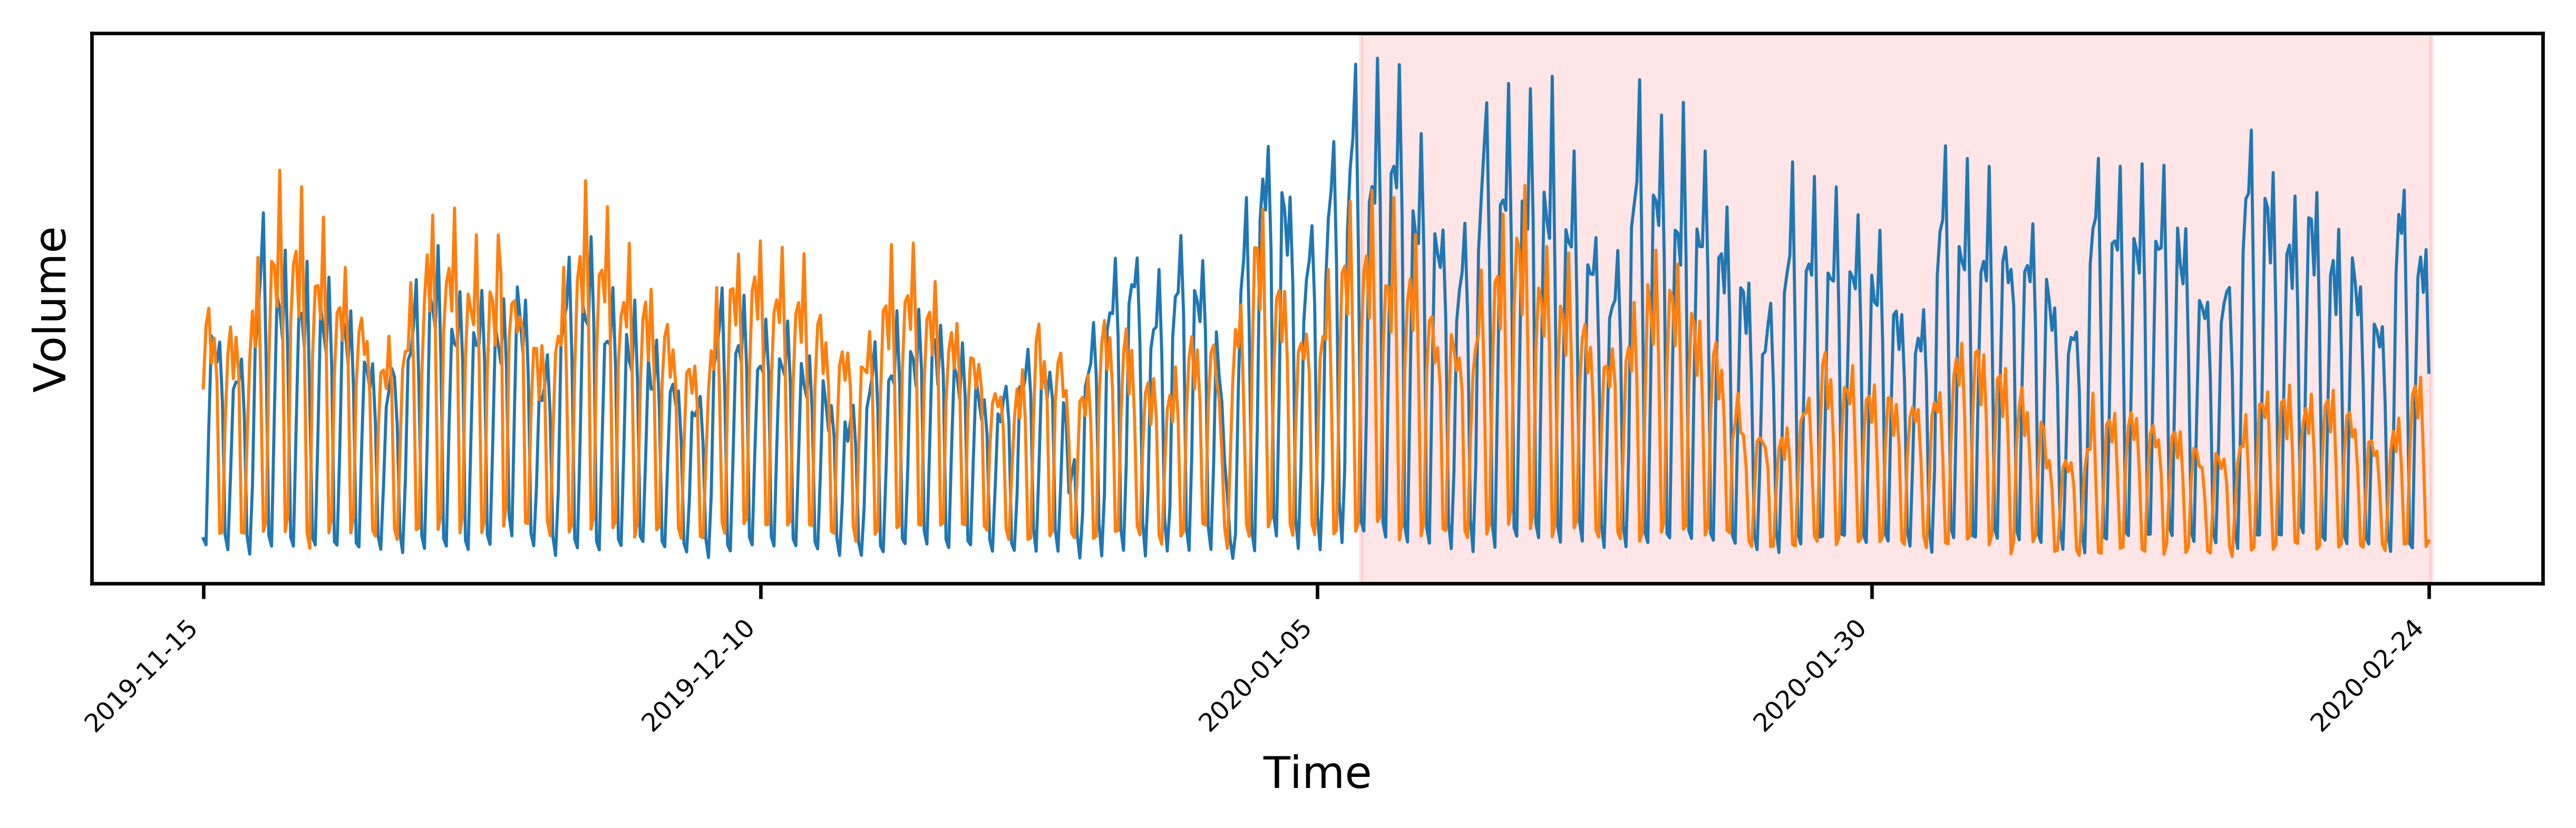
\includegraphics[width=1.1\textwidth, scale=1.5]{asi_cov_3.png}}}{\caption{Skyscanner - Early effects of COVID-19 on travel demand in Asia (Singapore - orange, Poland - blue)}\label{fig:skyscanner1}}
	\end{floatrow}
	\begin{floatrow}
	  \ffigbox[\textwidth]{\makebox[\textwidth][c]{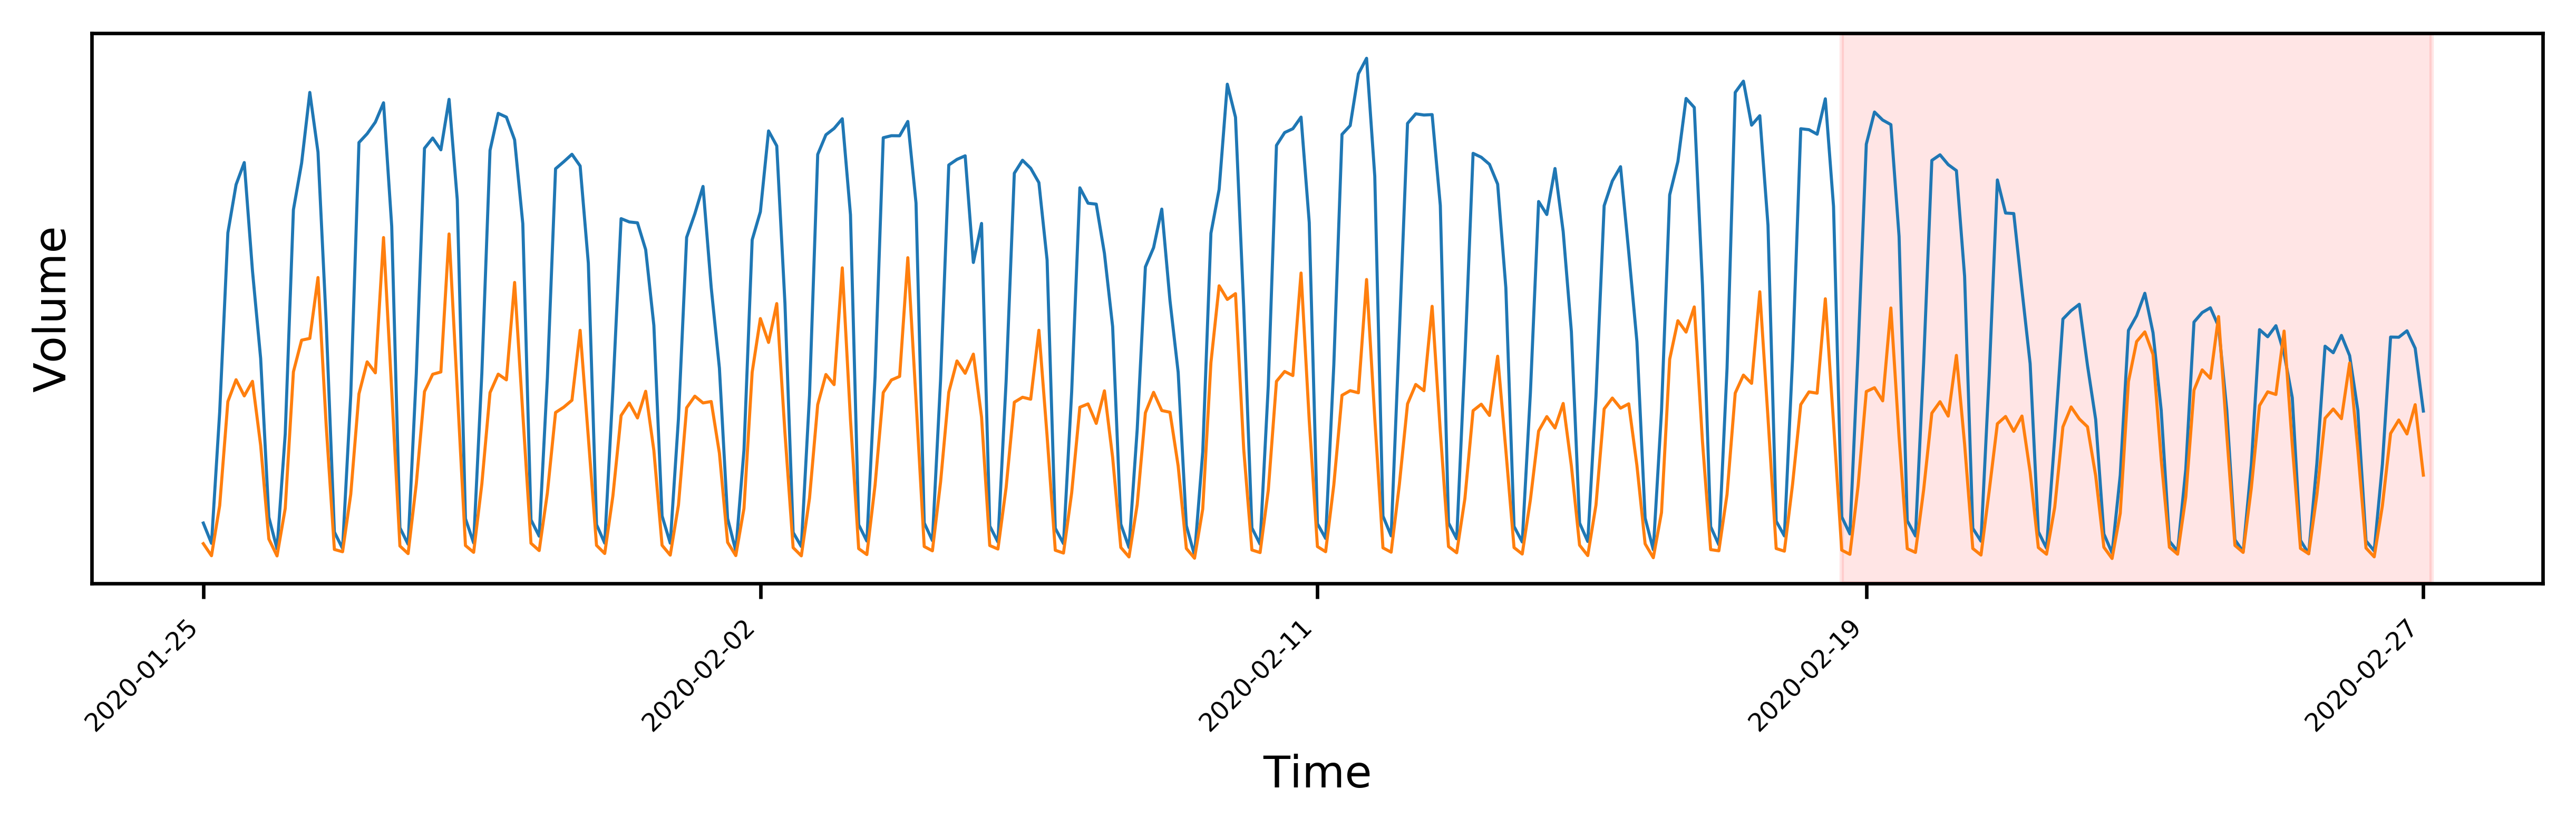
\includegraphics[width=1.1\textwidth, scale=1.5]{it_cov_3.png}}}{\caption{Skyscanner - Early effects of COVID-19 on travel demand in Italy (in blue, compared with the Netherlands in orange)}\label{fig:skyscanner2}}
	\end{floatrow}
\end{figure}

This research focused on the application of anomaly detection to Skyscanner's ``redirects'' dataset, which records when users redirect to partner websites, and is a way of gauging demand in the market.

The raw dataset is a large, heterogeneous dataset of individual events. In order to extract meaningful information from it, it has to be integrated and summarised over time windows. Given the redirects dataset's scale, this transformation was applied using an ETL job developed with Apache Spark.

The redirects dataset is highly periodic, and has several trends that appear. The types of anomalies that can be found in the dataset are mainly \textit{contextual} anomalies, that are subtle deviations from normal.

It should be noted that more obvious group or point anomalies may occur in the data, but these are mostly due to errors and are usually ``backfilled'' to correct them, so it is difficult to get an example of these kinds of anomalies in hindsight. 

In Figures \ref{fig:skyscanner1} and \ref{fig:skyscanner2}, the precise $y$-axis values have been redacted so as to conceal commercially sensitive information, however they are both on the same scale and represent the same metric for users in different markets. These particular series were chosen as one series is nominal and one series is anomalous in each figure, and they provide a fair comparison to identify an anomaly in context. In Figure \ref{fig:skyscanner1}, one can clearly detect that the orange line is anomalous as it falls significantly below the trend in the right half of the figure. In Figure \ref{fig:skyscanner2}, the blue line (Italy) experiences a significant anomalous drop at the end. Both Figure \ref{fig:skyscanner1} and \ref{fig:skyscanner2} are examples of contextual anomalies. It could be argued that there is a point which is anomalous in Figure \ref{fig:skyscanner2} and therefore it is a point anomaly, but the subsequent points are also anomalous given the context of the previous values of the series.

Figure \ref{fig:skyscanner1} is also an example of \textit{heteroskedasticity}, where in approximately the last third of the graph, the variance in the data is reduced, and this becomes the ``new normal''. There is a danger of misclassifying this ``new normal'' as normal despite it being anomalous. The graphed anomaly is long in duration, and so this is a potentially contentious decision for manual labelling - it is not clear if the entire second half of the graph should be labelled as anomalous, or just the two main points where the anomaly manifests itself in a change in peak values and variance.


\subsection{Sample Datasets}
In order to reason about any model's performance, this work uses publicly-available sample datasets with labelled anomalies in order to benchmark models. Several datasets were considered, with the goal of being as representative of the Skyscanner dataset as possible.

\subsubsection{Yahoo A1}

\begin{figure}[h]
	\graphicspath{{../code/notebooks/02_Sample_Dataset_Figures_output/}}
	\floatsetup{justification=centering,rowpostcode=myrowsep}
	\begin{floatrow}
	  \ffigbox[\FBwidth]{\makebox[\textwidth][c]{\includegraphics[width=1\textwidth]{yahoo_a1_series_1.png}}}{\caption{A point anomaly in Yahoo A1.}\label{fig:yahoo-point-anomaly}}
	\end{floatrow}
	\begin{floatrow}
	  \ffigbox[\FBwidth]{\makebox[\textwidth][c]{\includegraphics[width=1\textwidth]{yahoo_a1_series_17.png}}}{\caption{Group anomalies in Yahoo A1.}\label{fig:yahoo-group-anomaly}}
	\end{floatrow}
	\begin{floatrow}
	  \ffigbox[\FBwidth]{\makebox[\textwidth][c]{\includegraphics[width=1\textwidth]{yahoo_a1_series_37.png}}}{\caption{Contextual anomaly (Section \ref{section:types-of-anomalies}) in Yahoo A1.}\label{fig:yahoo-contextual-anomaly}}
	\end{floatrow}
	\begin{floatrow}
	  \ffigbox[\FBwidth]{\makebox[\textwidth][c]{\includegraphics[width=1\textwidth]{yahoo_a1_series_36.png}}}{\caption{Example of a periodic Pattern in Yahoo A1 with point anomalies.}\label{fig:yahoo-periodic-pattern}}
	\end{floatrow}
\end{figure}

The Yahoo \citep{YahooLabs} A1 benchmark dataset contains extracts from real Yahoo production data (obfuscated to conceal its true representation) which, after some transformation, can be categorised as a multivariate time-series dataset, consisting of 65 series and 1400 datapoints. The data is a real-world dataset, therefore it is representative of the Skyscanner data with intended application. 

Its anomaly labels are also very accurate and tightly-fit to the anomalous points. It contains examples of all the types of anomalies described in Section \ref{section:types-of-anomalies} - point (Figure \ref{fig:yahoo-point-anomaly}), group (Figure \ref{fig:yahoo-group-anomaly}) and contextual (Figure \ref{fig:yahoo-contextual-anomaly}). The dataset also has examples of different patterns, such as periodic, static, heteroskedastic and noisy. An example of a periodic pattern can be seen in Figure \ref{fig:yahoo-periodic-pattern}, which is similar to the shape of the Skyscanner redirects data. All of these criteria make the dataset very suitable to the problem at hand.

In Figures \ref{fig:yahoo-point-anomaly}, \ref{fig:yahoo-group-anomaly}, \ref{fig:yahoo-contextual-anomaly} and \ref{fig:yahoo-periodic-pattern}, it is not known precisely what the $y$-axis represents, all that is known is that these are extracts of real Yahoo production data. The $y$-axis values are simply denoted as ``value'' in the dataset. Presumably the true units have been concealed to not reveal commercially sensitive data.

The $x$-axis of Figures \ref{fig:yahoo-point-anomaly}, \ref{fig:yahoo-group-anomaly}, \ref{fig:yahoo-contextual-anomaly} and \ref{fig:yahoo-periodic-pattern} is given as an integer representing the time-step, starting from 1. It is not known what the frequency of these time-steps is.

Figure \ref{fig:yahoo-contextual-anomaly} shows an example of a contextual anomaly. The reason the highlighted points are anomalous in this context is due to the lack of low-valued points at this time interval, and the dense nature of the points. These points may be considered normal if treated in isolation, but the context of the earlier time-periods provides some indication that these points may be anomalous.

The only major issue with the Yahoo dataset is that the number of datapoints (1400) is relatively low for a machine learning model to be effective - this motivated the dataset being upsampled and interpolated in order to create more training examples.


\subsubsection{Numenta Anomaly Benchmark (NAB)}

\begin{figure}[h]
	\graphicspath{{../code/notebooks/02_Sample_Dataset_Figures_output/}}
	\floatsetup{justification =centering, rowpostcode=myrowsep}
	\begin{floatrow}
	  \ffigbox[\FBwidth]{\makebox[\textwidth][c]{\includegraphics[width=1\textwidth]{nab_tweets_FB.png}}}{\caption{NAB Tweets - FB - Point anomalies.}\label{fig:nab-point-anomaly}}
	\end{floatrow}
\end{figure}

The Numenta Anomaly Benchmark \citep{NAB} or NAB provides several time-series datasets, and also provides a framework for evaluating models on these datasets.

The ``tweets'' dataset is comprised of the volume of tweets relating to particular stock market stocks. This is a multivariate time-series with roughly 15,000 datapoints and 10 individual time-series. It is also seasonal and periodic, and as such is a suitable dataset for benchmarking on, as it matches the criteria of the Skyscanner data. The NAB Tweets dataset mainly has examples of point anomalies (as can be seen in Figure \ref{fig:nab-point-anomaly}).

Similar to the \textit{Yahoo A1} dataset, the NAB Tweets dataset also benefited from upsampling and interpolation, though with 15000 datapoints it was not as significant that this be done.

The other datasets in the NAB collection are either univariate or not representative of the Skyscanner dataset for envisaged application.

% Aim: 2 pages
%\clearpage
\section{The System}
\label{section:the-system}

\begin{figure*}[ht]
	\graphicspath{{img/}}
	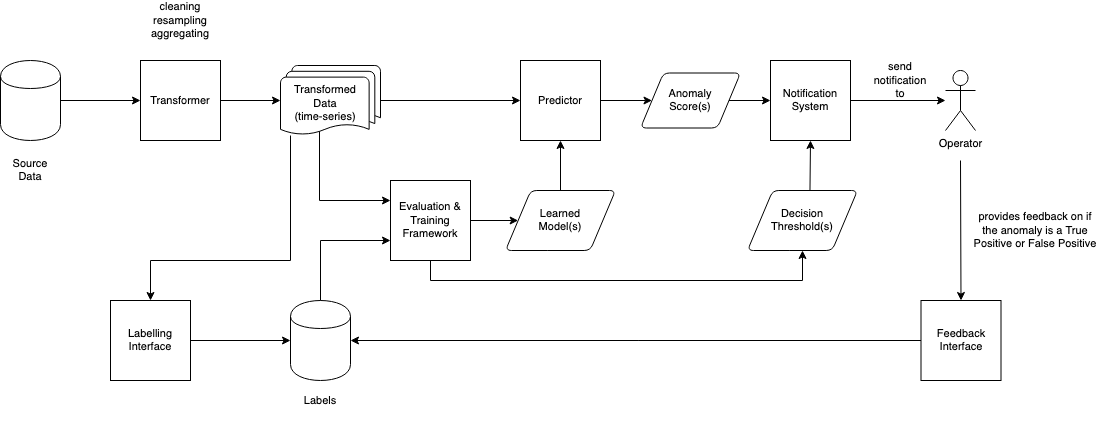
\includegraphics[width=\textwidth]{AnomalyDetectionSystemDesign.png}
	\caption{Proposed System Design Diagram}
	\label{fig:system-design}
\end{figure*}


\subsection{Overview}
Though the work described in this paper did not include the creation of a production-ready large-scale anomaly detection system, its aim is to determine the feasibility of building such a system and to make recommendations as to how such a system could be implemented, specifically in the context of Skyscanner. This section details these recommendations.

\subsection{Constraints}

\subsubsection{Scale}

Given the title ``large-scale anomaly detection system'', it is clear that the scale of the datasets the system must be able to run on is significant.

The Skyscanner redirects dataset (one of the intended target datasets of the system) is well within the territory of ``big data'', with millions of records being produced per day. The sheer volume of data warrants the use of distributed big data technologies such as Spark (expanded on below in Section \ref{section:distributed-vs-single-process}).

Given the volume of data, and the need to label it (see Section \ref{section:unlabelled-datasets}) the decision was taken to use sample datasets to approximate the redirects dataset. This allowed an experimental implementation to be created with Pandas\footnote{\url{https://pandas.pydata.org/}} and allowed for faster prototyping of models and anomaly detection techniques.

\subsubsection{Alerting Norms}

The need for meaningful alerts is discussed extensively in Section \ref{section:meaningful-alerts}, however it is important that it be called out as a key constraint on the system being acceptable in practice in Skyscanner. Alerts which do not serve their purpose are quickly silenced, so the \textit{precision} of trained models is especially important.

\subsubsection{Generalisation to other datasets}

In order for the anomaly detection system to have impact in a context like that of Skyscanner, it must have some ability to generalise to different datasets. It is important to note that the Transformer component (see Figure \ref{fig:system-design}) could be different for each dataset to transform the data into a representation which is optimal for the anomaly detection system. Models may be trained per-dataset so that each dataset may be modelled correctly. It would also be valuable for multiple datasets to be joined and collated into a multivariate time-series, that allows them to be modelled and predicted jointly, increasing the predictive potential of the system.

\subsection{System Design}

The recommended system architecture for the anomaly detection system can be seen in Figure \ref{fig:system-design}. The architecture diagram is generic and is intended to generalise the system's function, whether it were to use the streaming or batch paradigm (discussed in Section \ref{section:streaming-vs-batch}).

The data is assumed to already be ingested into a Data Source in a raw format, where the data is then transformed by the Transformer component. The transformation applied could be resampling, cleaning, aggregating or filtering, to name a few. The resulting transformed data should be in the format of a time-series. This time-series can be stored in an intermediate location (be that persistent storage or a separate data stream depending on the paradigm).

Initially, labels must be created for the data, using any of the methods discussed in Section \ref{section:unlabelled-datasets}. This could be accomplished via crowdsourcing, or simply manual inspection via a graphical interface. This is generalised by the ``Labelling Interface'' on the diagram. These labels, combined with the transformed time-series, are used to train and evaluate models using the Evaluation \& Training Framework. The outputs of this stage are the learned models and decision thresholds that can be used to classify anomalies.

In live evaluation mode, the transformed time-series data is given as input to the Predictor module which evaluates trained models and outputs anomaly score(s). The anomaly scores, combined with the learned decision threshold(s), are combined by the Notification System, to decide whether or not to alert an operator.

In order to employ online learning and continuously improve the anomaly detection system, any alerts sent to an operator should include instructions on providing feedback on the alert. This occurs via the Feedback Interface, and can, in this way, add labels for more up-to-date data, augmenting the training set and allowing future trained models to be more accurate.

The design is heavily inspired by Microsoft's \citep{MicrosoftTimeSeries} time series anomaly detection system, but is intended to be more generic to facilitate application to other tech stacks and paradigms.

\subsection{Design Choices}

\subsubsection{Real-time vs Batch}
\label{section:streaming-vs-batch}

There are several convincing arguments for using both real-time and batch processing paradigms to implement the anomaly detection system, and this could have significant implications for the applicability and usage of the system.

Using the real-time (or streaming) paradigm, anomaly detection could occur on data at a much finer granularity, allowing for a prompt response to new, developing anomalies (say, within 5 minutes). This would be useful in detecting production incidents and live software issues, but could be limited in its ability to identify long-term, systemic or trend anomalies happening over a larger timeframe. The real-time paradigm would also add complexity to the system, in the form of handling data replays, and persisting the streaming data for use in training - though realistically, it is likely that it would be available in archives, as would be the case in Skyscanner.

Using the batch paradigm, extremely quick responses (e.g. sub 5 minutes) would not be possible, however, in practical terms this may not matter. Traditional monitoring systems with thresholds can detect fast-occurring issues. The added value of having an anomaly detection system would be to identify larger, or more subtle medium-to-long-term anomalies. Using the batch paradigm reduces complexity as evaluation is done in a cron-based or offline manner, and there are many ETL platforms able to facilitate this. It also allows more complex or computationally-expensive models to be used as they can take much longer to complete, and less focus can be given to the optimisation of the training code.

\subsubsection{Distributed vs single-process}
\label{section:distributed-vs-single-process}

Given that the system should be able to cope with large-scale datasets, this would motivate the use of distributed big data technologies like Apache Spark, which is extensively used in Skyscanner. Spark offers PySpark which has a Dataframe interface similar to that of the Pandas library. Though there is some similarity, Pandas is much more featured and allows for faster prototyping, and therefore Pandas was used in the creation of the evaluation framework for this work, to derive the results from different models.

When implementing the system, the experimental code created would have to be migrated to use Spark dataframes rather than Pandas, and this would allow large datasets that cannot fit on one node to be used as inputs.

\subsubsection{Root Cause Identification}

Once an anomaly alert is created and sent to an operator, the operator must respond, by analysing visualisations and/or debugging the system state, to determine the nature of the anomaly. Ultimately the operator's goal is to identify the root cause of the anomaly and address the problem or respond appropriately. 

Though it is unlikely that the system could fully identify the root cause, one way in which the system could assist with this is by identifying the specific time-series that has caused the anomaly alert to be created. However, by reducing the problem to individual series, we remove the multivariate element of the data and therefore predictions and scores may be less accurate overall.

In order to overcome this for our prediction models (Section \ref{section:prediction-models}), a mixed approach of multivariate prediction with univariate scoring may be used, where the prediction model makes predictions taking all time-series into account, but the computed errors are used to model individual univariate normal distributions for each time-series, allowing each series to have an anomaly score and alerts to be created for individual series.

\cite{deepMultivariateNetwork} identify root cause identification as one of their contributions, and that their MSCRED framework jointly addresses the issues of anomaly detection, root cause identification and anomaly severity. Implementing MSCRED may be an area for future work.

\subsubsection{Ensemble Methods}

Given that there are several models evaluated in this work, it may be possible to create better anomaly scores by combining the output of multiple models, also known as using \textit{ensemble methods}. This approach is also recommended by \cite{MicrosoftTimeSeries} as future work. The merging of results could be a mean average, maximum, or percentile. It should be noted that this would require the decision threshold to be treated separately from that of the individual models.

Different models may output anomaly scores with different variances, and so the anomaly scores may not lend themselves to combination with a single decision threshold in this way. Alternatively, each model may have its own decision threshold and ``vote'' for normal (0) or anomalous (1). With an odd number of models, a consensus may always be reached by the ensemble.

To further improve predictions, a weighting may be added to each of the ensemble models, to favour more accurate models and reduce the overall impact of noisy model outputs.


\subsection{Maintenance \& Operation}

The ongoing maintenance and operational costs associated with running a large-scale anomaly detection system would be mainly around re-training and continuous improvement. Given that the anomaly detection system's purpose is to monitor the data produced by other systems, it is important that it, too, is reliable.

By the nature of the design, there is a feedback loop in place for continuous labelling of alerts as true anomalies or false positives, which allows for training sets to be augmented. Periodically, the model's performance should be reviewed by data scientists, and adjustments to hyper-parameters made to optimise its performance in an ongoing manner.

% Evaluation
\section{Evaluation}
\label{section:evaluation}

\subsection{Metrics \& Evaluation Framework}
\label{section:evaluation-metrics-framework}

As discussed at length in Section \ref{section:meaningful-alerts}, it is important that an anomaly detection system trade-off between precision and recall, and this is achieved using the $F_\beta$-score.

Given the importance of producing \textit{meaningful} alerts, the system should balance between precision and recall. 
%To achieve this, the chosen value of $\beta$ has to be in the interval $0 < \beta < 1$.
\cite{lstmTimeSeriesAnomalyDetection} use $\beta \ll 1$ to give more weight to precision, however, in the end, a value of $\beta = 1$ was chosen for this work as it allowed for better optimisation of the decision threshold.

In order to evaluate different models, an evaluation framework was constructed, using mainly Pandas and Numpy\footnote{\url{https://numpy.org/}}. The framework evaluates models by splitting the sample datasets into training and cross-validation sets. K-fold methods were not used due to the nature of time-series having to remain ordered. It is not intuitive to use datapoints earlier than the training data as a cross-validation set, since the problem consists of forecasting future anomalies based on past data.

The evaluation framework also evaluates the models performance on cross-validation sets at varying degrees of synthetic contamination in the training set, ranging from 0\% to 5\%, inspired by \cite{DAGMM}'s approach. As discussed in Section \ref{section:incorrect-labels-contaminations}, this provides an indication into the model's robustness to \textit{some} incorrect labelling in the training data.

The framework runs training on each of the models, then uses the outputs of the trained model on the training set to optimise a threshold parameter, using the $F_\beta$-score as the function to maximise (in reality, minimise $1 - F_\beta$) with the choice of threshold parameter. This is similar to the approach of the Numenta Anomaly Benchmark.

For every run, the performance metrics for the model are computed - namely the precision, recall and $F_\beta$-score. These metrics were chosen because higher scores in these metrics equate better business outcomes. A higher recall indicates identification of more correct anomalies, which is, of course, desirable. A higher precision indicates that there is a higher chance of every alert raised by the model actually corresponding to a true anomaly. A higher $F_\beta$-score trades off the performance gains of the former two metrics.

In addition to comparing different models' performance metrics, the models will also be evaluated on their characteristics - for example, deep learning models tend to improve with larger training sets.

\subsection{Models}

In order to perform anomaly detection, the system must utilise the best model for the problem. As such, several models were evaluated, and they are described here. 

\subsubsection{Last Value}

In order to benchmark more complicated models, this work uses a simple prediction model using the previous value for every timestep as the prediction. During training, the model fits a normal distribution over the squared errors using this prediction. This normal distribution's CDF is evaluated for the squared prediction error at each point, to produce the probability of the observation being anomalous. This model is intended purely as a naive benchmark and would not be used in practice.

\subsubsection{ADSaS}

ADSaS is a time-series analysis model developed by \cite{ADSaS} which makes the claim that it is more performant than machine-learning-based models, like LSTM, in terms of precision, recall and $F_1$-score. Given that the work is critical of LSTM, ADSaS is a good model for comparison, given this work also implements LSTM.

ADSaS is a combination of two main time-series analysis methods - Seasonal Auto-Regressive Integrated Moving Average (SARIMA) and Seasonal Trend Decomposition using LOESS (STL). The former is a prediction model which has a seasonality parameter and is adapted to non-stationary data with a seasonality. This prediction is then differenced with the real values to compute the error, and this error is decomposed with STL. The \textit{residuals} of the decomposition are then collected and modelled as a normal distribution, and the CDF used as the anomaly score, as described in Section \ref{section:prediction-models}.

\begin{figure}[h]
	\graphicspath{{img/}}
	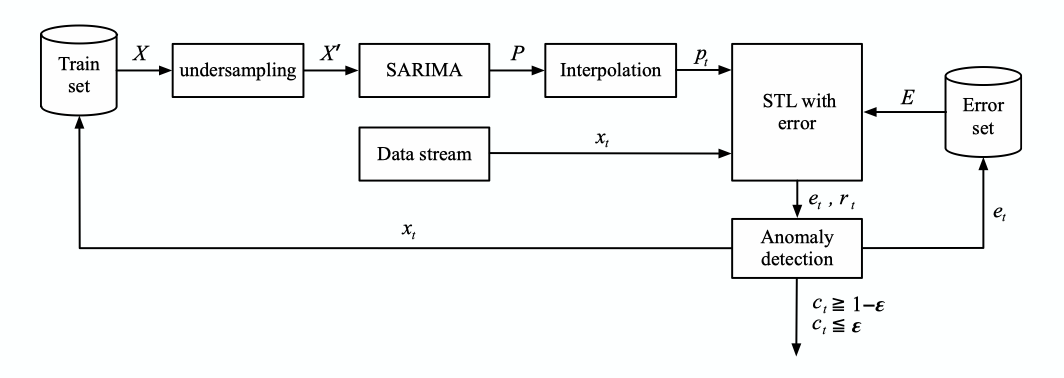
\includegraphics[width=\textwidth]{adsas_diagram.png}
	\caption{ADSaS diagram from \cite{ADSaS}}
	\label{fig:adsas-diagram}
\end{figure}

In the original implementation, under-sampling and interpolation steps are also used around the SARIMA model (as can be seen in Figure \ref{fig:adsas-diagram}), but these were ommited as the data was not - when evaluating on the sample datasets - on a scale that warranted under-sampling.


\subsubsection{LSTM}

The LSTM model is an LSTM recurrent neural network that outputs a prediction given $n$ previous timesteps of observations. The full specification of LSTM and the training algorithm Backpropagation Through Time (BPTT) can be found in \cite{LSTMHochreiter}. For the purposes of this evaluation, the model was implemented using the Keras\footnote{\url{https://keras.io/}} library.

LSTM networks function using multiplicative gates that enforce constant error flow through the internal states of special time units called ``memory cells'' \citep{lstmTimeSeriesAnomalyDetection}. This allows them to learn long-term correlations in data and model complex multivariate sequences.

In the simple LSTM model, normal distributions were fit around the squared prediction errors, individually for each series in the input, and the CDF used to generate anomaly scores in the evaluation step of the model lifecycle.

\subsubsection{LSTM + STL}

In addition to LSTM, a combination of the ADSaS and LSTM approaches is achieved with the LSTM + STL model. The intuition is similar to that of ADSaS, in the way of using the STL-decomposed residuals of prediction errors to produce anomaly scores, but the prediction itself is done by an LSTM neural network.

\subsection{Results}

\begin{figure*}[h]
\begin{center}
	\caption{Comparison of $F_\beta$-score, precision and recall across datasets by model}
	\label{fig:results-model-comparison}
	\begin{tabular}{c|ccc|ccc}
		\hline
		& \multicolumn{3}{c|}{\textbf{NAB Tweets}} & \multicolumn{3}{c}{\textbf{Yahoo A1}} \\
		\textbf{Model} 
		& $F_\beta$-score & Precision & Recall
		& $F_\beta$-score & Precision & Recall
		\\
		\hline
		&&&&&&\\
		\csvreader[head to column names]{../code/evaluation/output/model_comparison_on_datasets.csv}{}{
			\model 
			& \csvcolii & \csvcoliii & \csvcoliv
			& \csvcolv & \csvcolvi & \csvcolvii
			\\ 
		}
		&&&&&&\\
		\hline
		\textbf{Best} & LSTM+STL & LSTM+STL & LSTM & LSTM+STL & LSTM+STL & ADSaS \\
	\end{tabular}
\end{center}
\end{figure*}

%Figure 2: sectioned for each dataset, for each level of contamination, score for each model
\begin{figure*}[h]
\begin{center}
\caption{Model robustness to contamination}
\label{fig:results-contamination}

\subfloat[Yahoo A1]{
	\begin{tabular}{c|ccc|ccc|ccc}
		\hline
		\textbf{Contamination (\%)} & \multicolumn{3}{c|}{\textbf{ADSaS}} & \multicolumn{3}{c|}{\textbf{LSTM}} & \multicolumn{3}{c}{\textbf{LSTM + STL}} \\
		 & Precision & Recall & $F_\beta$-score %& TP 
		 & Precision & Recall & $F_\beta$-score %& TP 
		 & Precision & Recall & $F_\beta$-score %& TP 
		 \\
		\hline
		\csvreader[head to column names]{../code/evaluation/output/contmination_comparison_yahoo_a1.csv}{}{
			\contamination 
			& \csvcoliii & \csvcoliv & \csvcolii %& \csvcolv 
			& \csvcolvii & \csvcolviii & \csvcolvi %& \csvcolix 
			& \csvcolxi & \csvcolxii & \csvcolx %& 0 
			\\ 		
		}
		&&&&&&
		\\
	\end{tabular}
}
\\
\subfloat[NAB Tweets]{
	\begin{tabular}{c|ccc|ccc|ccc}
		\hline
		\textbf{Contamination (\%)} & \multicolumn{3}{c|}{\textbf{ADSaS}} & \multicolumn{3}{c|}{\textbf{LSTM}} & \multicolumn{3}{c}{\textbf{LSTM + STL}} \\
		 & Precision & Recall & $F_\beta$-score %& TP 
		 & Precision & Recall & $F_\beta$-score %& TP 
		 & Precision & Recall & $F_\beta$-score %& TP 
		 \\
		\hline
		\csvreader[head to column names]{../code/evaluation/output/contmination_comparison_nab_tweets.csv}{}{
			\contamination 
			& \csvcoliii & \csvcoliv & \csvcolii %& \csvcolv 
			& \csvcolvii & \csvcolviii & \csvcolvi %& \csvcolix 
			& \csvcolxi & \csvcolxii & \csvcolx %& 0 
			\\ 
		}
		&&&&&&&&\\
	\end{tabular}
}

\end{center}
\end{figure*}

\subsubsection{Model Comparison Results}
\label{section:model-comparison-results}

Figure \ref{fig:results-model-comparison} shows the comparison of the $F_\beta$-score, precision and recall obtained on each dataset (with no contamination) for each evaluated model, and shows which model obtained the best score for each metric.

As can be seen from the results, the LSTM + STL model was the highest scoring model for precision and $F_\beta$-score on both datasets. Given the importance of creating meaningful alerts, this implies that the best model of all the models compared was LSTM + STL.

The plain LSTM model achieved the highest recall on the NAB dataset by quite some margin. ADSaS achieved higher recall on the Yahoo A1 dataset, but not by as much comparatively to LSTM which had a lower but similar score.

\subsubsection{Contamination Results}
\label{section:contamination-results}

Figure \ref{fig:results-contamination} shows the precision, recall and $F_\beta$-score of each model, split by dataset, at varying degrees of contamination (as discussed in Section \ref{section:evaluation-metrics-framework}). The contamination \% refers to the \% of the \textit{training} set that was contaminated, whereas the metric results are the results of the same model on the \textit{cross-validation} set.

Though the results are not as clean as would intuitively be expected, they do show that overall recall tends to drop as contamination increases, suggesting the model is less able to accurately predict anomalies. However, precision seems to show an increasing trend, which is counter-intuitive. 

This could be because the total positive predictions (true positives $+$ false positives) is reduced due to the model learning less precise decision boundaries due to the contamination, and therefore gives less overall positive guesses. By reducing TP+FP comparatively more than TP alone, precision improves, given that TP+FP is the denominator of precision. Further investigation is required to understand why this occurs and if the model(s) are overfitting at 0\% contamination.

The contamination results do not conclusively say which model is most robust to incorrectly labelled training sets. On the Yahoo A1 results, if considering recall as the metric to evaluate on, the reduction in recall from 0\% to 5\% contamination in the ADSaS results was the most significant and in LSTM+STL was the least significant. This provides \textit{some} indication that LSTM+STL may cope with contaminations better, but further experimentation would be required, perhaps with different datasets, to prove this conclusively.

\subsubsection{Experimental Critique / Improvements}

The reported precision, recall and $F_\beta$-scores were computed on the flattened predictions and actual values across all series. However, by inspecting the values of the metrics on each series and taking the maximum or average of these, better results could be reported. However, the single computation on flattened results gives more robust results.

\subsubsection{Comparison of characteristics}

The LSTM-based models (LSTM and LSTM + STL) are deep learning models, and therefore their performance metrics (precision, recall, $F_\beta$-score) tend to improve given larger training datasets. The ADSaS model is a simple time-series analysis model, whose performance would not be significantly improved given more training data.

The LSTM models take more time to train (unless specific hardware acceleration is used) and are more computationally expensive, however produce more accurate predictions. The ADSaS model can be trained quickly and in real-time - though this is not a major consideration for application in Skyscanner.

All evaluated models can be thought of as \textit{semi-supervised} models, which learn normal values and thresholds around those, therefore are better able to learn a representation of normal with more data as it is added, therefore all of the models lend themselves to online learning and re-training over time. However, the deep learning LSTM models would see more of a performance increase from continuous re-training and online learning.

% Related Work
% Aim: 1-2 pages
%\clearpage
\section{Related Work}

The field of applied time-series anomaly detection has seen several works in recent years, focusing on different techniques such as temporal prediction methods, Convolutional Neural Networks (CNNs), LSTM and density estimation methods. This section explores some alternative anomaly detection methods.

\subsection{Convolutional Neural Networks (CNNs)}
\label{section:cnn}

\cite{deepMultivariateNetwork} and \cite{MicrosoftTimeSeries} are examples of works where CNNs are applied to time-series anomaly detection. Both works have similarities and differences in their approach.

Both works do not apply Convolutional Neural Networks directly to the input data - they instead transform the data into a spatially-significant representation.
In the MSCRED framework described by \cite{deepMultivariateNetwork}, the multivariate time-series are collated into ``system signature matrices'' by computing the inner product of two time-series, for every pair of time-series. This allows for two-dimensional convolution operations to be applied to these matrices and makes the model more robust to noise. The signature matrices allow the correlations between different pairs of time-series to be captured. \cite{deepMultivariateNetwork} reference previous studies stating these are critical to characterise system status.

In \cite{MicrosoftTimeSeries}, the \textit{Spectral Residual} transform, a simple yet powerful approach based on \textit{Fast Fourrier Transform (FFT)} \citep{MicrosoftTimeSeries}, is applied to the input data to produce a ``saliency map''. This saliency map is then given as input to one-dimensional convolutional layers of a CNN. \cite{MicrosoftTimeSeries} state that this is because of the lack of labelled data - by transforming the data into a saliency map, the CNN can be trained on saliency maps, which is a much more constrained domain and yield better results when the labels are lacking.

Both \cite{deepMultivariateNetwork} and \cite{MicrosoftTimeSeries} also use a combination of real and synthetic data for training. 
\cite{MicrosoftTimeSeries} use real production time-series augmented with synthetic anomalies as training data. This is done because of the problem of lack of labelled data mentioned as the main challenge in their paper. By utilising production data as the basis, they aid their model to learn ``normal'' behaviours.
\cite{deepMultivariateNetwork} evaluate their model on both synthetic data and a real-world power plant dataset. Their synthetic data is completely synthetic, generated based on a sinusoidal pattern with noise.

The works differ in the case of their expected output - \cite{MicrosoftTimeSeries} only wish to be able to identify if a given window of points is anomalous, however \cite{deepMultivariateNetwork} concern themselves also with \textit{anomaly diagnosis}, pointing out which time-series are to blame for the anomaly and the precise point at which the anomaly occurs.

There is generally a consensus that convolutional neural networks require some transformation of the input data, such that convolution operations are effective on the representation.

\subsection{Temporal prediction methods}
\label{section:temporal-prediction-related-work}

Temporal prediction methods operate on the intuition of detecting deviation-based outliers of specific time-instants with the use of regression-based forecasting models - outliers are declared on the basis of deviations from expected (or forecasted) values \citep{outlierAnalysisBook}.

Temporal prediction methods rely on the principle of \textit{temporal continuity}, which assumes that patterns in the data are not expected to change abruptly, unless there are abnormal processes at work \citep{outlierAnalysisBook}.

\cite{outlierAnalysisBook} states that the regression models used in temporal methods can utilise correlations both across time (referring to temporal continuity) or across series, as many applications output multivariate time series that are often closely correlated with one another.

Conventional time-series analysis methods often do not perform well in anomaly detection, or find anomalies in limited conditions \citep{ADSaS}. For example, SARIMA and STL, are used only for stationary and periodic time-series respectively \citep{ADSaS}, but in the ADSaS system \citep{ADSaS}, combining STL and SARIMA is shown to detect anomalies with high accuracy for data that is even noisy and non-periodic.

ARIMA (Auto-Regressive Integrated Moving Average) models generalise the simplest time-series forecasting models. Autoregressive (AR) models predict the next point in a time-series based on a weighted combination of a given number of previous terms in the time-series. Moving Average (MA) models predict the next point based on a given number of previous \textit{white noise} terms.

$$ AR(p): X_t = \sum_{i=1}^{p} a_i \cdot X_{t-i} + c + \epsilon_t $$ 
\citep{outlierAnalysisBook}

$$ MA(q): X_t = \sum_{i=1}^{q} b_i \cdot \epsilon_{t-i} + \mu + \epsilon_t $$ 
\citep{outlierAnalysisBook}

$$ ARMA(p, q): X_t = \sum_{i=1}^{p} a_i \cdot X_{t-i} + \sum_{i=1}^{q} b_i \cdot \epsilon_{t-i} + c + \epsilon_t $$ 
\citep{outlierAnalysisBook}

The ARMA model can be enhanced to capture persistent trends with the ARIMA model (Auto Regressive Integrated Moving Average), which works better for such \textit{non-stationary} time series \citep{outlierAnalysisBook}.

STL is a versatile and robust method for time-series decomposition \citep{ADSaS}. It is an algorithm developed to decompose a time-series into three components. Namely, the trend, seasonality and residuals. The trend shows a persisting direction in the data, seasonality shows seasonal factors and residuals show the noise of the time-series \citep{ADSaS}.

%\cite{outlierAnalysisBook} and \cite{ADSaS} both are high quality works that give insight into temporal prediction methods. \cite{outlierAnalysisBook} is a textbook covering the fundamentals of time-series prediction methods applied to outlier analysis and \cite{ADSaS} is a research paper combining multiple time-series prediction methods to have better performance than many state-of-the-art deep learning approaches, suggesting that it is worth considering purely statistical time-series analysis models as a viable option for anomaly detection.

\subsection{Density Estimation}

Density estimation is a popular technique that has been utilised in anomaly detection. Anomaly detection itself \textbf{\textit{is}} density estimation - given many input samples, anomalies are samples that reside in low probability density areas \citep{DAGMM}.

One of the main problems with density estimation is the \textit{curse of dimensionality} (see Section 
\ref{section:curse-of-dimensionality}) which motivates the use of dimensionality reduction techniques, like Principal Component Analysis or Autoencoders, coupled with density estimation. Most approaches focus on dimensionality reduction followed by density estimation, however they suffer from decoupled model learning with inconsistent optimisation goals and incapability of preserving essential information in the low-dimensional space \citep{DAGMM}. The DAGMM (Deep Autoencoding Gaussian Mixture Model) model proposed by \cite{DAGMM} provides an approach which uses an autoencoder and Gaussian Mixture Model, jointly optimising the parameters of the autoencoder and mixture model simultaneously in an end-to-end fashion.

%\cite{DAGMM}'s work provides a high-quality evaluation across several datasets, and benchmark comparisons against other density estimation and semi-supervised anomaly detection techniques, specifically introducing \textit{contaminated} datasets and assessing model performance on these. It shows an understanding of the field of density estimation anomaly detection techniques and it points to several other works which could be considered and further expored in future.

\subsection{Long-Short Term Memory (LSTM)}

Anomaly detection techniques involving LSTM deep neural networks are becoming popular in the field.

\cite{lstmEncoderDecorder} present an ``LSTM Encoder-Decorder'' (autoencoder) model for detecting anomalies in sensor data from machines, engines, vehicles etc. It is an example of an application of modern anomaly detection to a more traditional, established application of anomaly detection (mechanical engineering). The article states that unmonitored environmental conditions or load may lead to inherently unpredictable time-series. Detecting anomalies in such scenarios becomes challenging using standard approaches based on mathematical models that rely on stationarity, or prediction models that utilise prediction errors to detect anomalies. This motivates the use of a more advanced model like an LSTM autoencoder.

The model presented in \cite{lstmEncoderDecorder} consists of two neural networks, an Encoder and Decoder, which are chained together to form an autoencoder that is trained to reconstruct instances of normal time-series. As such, this can be considered a semi-supervised technique. \cite{lstmEncoderDecorder} explicitly mention that this is useful in scenarios when anomalous data is not available or is sparse. This is the case in their application as ``the relevant information pertaining to whether a machine is laden or unladen may not be available''. This is similar to the problem the research intends to solve wherein the anomalies are largely unknown and labels for the anomalies are not immediately available.

The work by \cite{lstmEncoderDecorder} is based on previous work by some of the same authors. \cite{lstmTimeSeriesAnomalyDetection} introduce LSTM neural networks to time-series anomaly detection, but rather than using them as an autoencoder, it uses a ``stacked LSTM based prediction model'', and then uses prediction errors on a training set to build a probability distribution of errors, which is then used to output a probability representing the anomaly score for a given time-step, and, combined with a decision threshold, can output binary anomaly labels. \cite{lstmTimeSeriesAnomalyDetection} also mention that by giving the network features that are ``control variables'' (features describing the settings chosen on manual operator controls) the network learned normal usage patterns, and was able to recognise anomalous control input as well as anomalous outcomes. 
%This is applicable to the Skyscanner datasets as configurations for various partners and areas of the business change frequently, so the model may want to learn the typical configuration changes that take place.

%Malhotra et al. appear to be the pioneers of LSTM application to time-series anomaly detection, and their work is comprehensive and clearly shows the results and value of their research.

Unfortunately, in the ADSaS system, \cite{ADSaS} point out several criticisms of LSTM models. The ADSaS system is designed to be real-time and is memory constrained to work on IoT devices, therefore the large training time and memory complexity of a deep learning model like LSTM is listed as a disadvantage when compared to conventional time-series forecasting methods. They also observe a better overall performance in the ADSaS system based on SARIMA and STL (discussed in Section \ref{section:temporal-prediction-related-work}). However, the main critique of this finding is that the evaluation of the algorithm was conducted on univariate time-series, and it is acknowledged in the conclusion that future work is required to apply the algorithm to multivariate time series, whereas it is known that LSTM performs well on multivariate data. \cite{ADSaS} also recognise that LSTM had the lowest prediction error compared to other algorithms - due to the fact that they adjust quickly to the norm after an abrupt change in pattern.

\subsection{Large-scale application of anomaly detection}

There are not many examples of research detailing the application of anomaly detection to large-scale datasets in a real-world context.

\cite{MicrosoftTimeSeries} describe Microsoft's implementation of time-series anomaly detection, which operates on the scale of 10,000 to 100,000 datapoints per second. The system is split into three major components: data ingestion, experimentation platform and online compute. The system is based around streaming real-time data in Apache Kafka processed by Apache Flink. Data is first ingested from a source and pushed into Kafka. The data is then evaluated by the ``online compute'' component. Finally, the experimentation platform allows researchers to train models and deploy them, validating their efficacy using evaluation metrics.

\cite{MicrosoftTimeSeries}'s system monitors minute-level time series, and is used by more than 200 product teams within Microsoft. This work therefore also is subject to the challenges discussed in Section \ref{section:meaningful-alerts} on creating meaningful alerts. There is also the problem of determining which is the correct team or person to alert for a given anomaly. There are many parallels between Microsoft's use case and the use case of this work in Skyscanner.

\cite{deepMultivariateNetwork}'s MSCRED framework also details an application of anomaly detection, as it was intended for use on data from a power plant. Though this is a real-world application of a significant scale, it is not comparable in terms of scale to Microsoft's anomaly detection system, or to the target dataset for this work.

% Future Work
% Aim: less than one page
\section{Future Work}

There are many areas for future research on anomaly detection techniques that could be applied.

First of all, the Convolutional Neural Network models discussed in Section \ref{section:cnn} have not been evaluated and compared with the prediction models, which could be beneficial in determining if CNNs could provide better performance for a large-scale anomaly detection system.

The LSTM-based model's performance could potentially be improved by jointly learning the correct prediction values as well as the decision threshold, letting it be dymanic and better cope with \textit{heteroskedasticity} (Section \ref{section:heteroskedasticity}).

Another area of future research could be in root cause identification and anomaly severity scoring. By capturing qualitative information or market sentiments, anomalies could be classified as system errors or genuine observed anomalies.

% Conclusions
% Aim: less than one page
\section{Conclusions}
\label{section:conclusions}

In this paper, various models are evaluated for application to a large-scale time-series anomaly detection system, whose design is proposed (Section \ref{section:the-system}).

The LSTM+STL model was chosen as the recommended model for the system to use, based on the fact that its precision and $F_\beta$-score results were the best of all the evaluated models (Section \ref{section:model-comparison-results}; Figure \ref{fig:results-model-comparison}) and there was some indication that it is more robust to incorrect labelling (Section \ref{section:contamination-results}). In addition, due to LSTM+STL being a machine-learning based model, it would be expected to become more accurate the larger the training set, and so it would be expected that its performance improve when applied to the full dataset, relative to that on the sample datasets.

This paper concludes that anomaly detection is feasible within the context of Skyscanner, and details how this could be accomplished, with a system design and model recommendation, serving as a blueprint for its implementation, that could be used as a reference point for similar use cases.


\vskip8pt \noindent
{\bf Project Code}

All code (except code for creating Figures \ref{fig:skyscanner1} and \ref{fig:skyscanner2}, which is Skyscanner-internal) for this project can be found at: \\ \url{https://github.com/pm990320/masters}.

%Access may be requested by emailing \\ \href{mailto:2250066m@student.gla.ac.uk}{2250066m@student.gla.ac.uk} or \href{mailto:patrickmenlove@hotmail.co.uk}{patrickmenlove@hotmail.co.uk}.

%% Acknowledgments
\vskip8pt \noindent
{\bf Acknowledgments}
\\Prof. Roderick Murray-Smith and Adam Kurkiewicz for supervising the research. \\ Dr Christos Anagostopolous for his assistance in the field of anomaly detection. \\ Skyscanner Ltd for their continued support of the research.


% Bibliography
\bibliographystyle{plainnat}
\bibliography{dissertation}

\end{document}
